%%
%% This is file `sample-acmtog.tex',
%% generated with the docstrip utility.
%%
%% The original source files were:
%%
%% samples.dtx  (with options: `acmtog')
%% 
%% IMPORTANT NOTICE:
%% 
%% For the copyright see the source file.
%% 
%% Any modified versions of this file must be renamed
%% with new filenames distinct from sample-acmtog.tex.
%% 
%% For distribution of the original source see the terms
%% for copying and modification in the file samples.dtx.
%% 
%% This generated file may be distributed as long as the
%% original source files, as listed above, are part of the
%% same distribution. (The sources need not necessarily be
%% in the same archive or directory.)
%%
%% The first command in your LaTeX source must be the \documentclass command.
\documentclass[acmtog]{acmart}
%% NOTE that a single column version is required for 
%% submission and peer review. This can be done by changing
%% the \doucmentclass[...]{acmart} in this template to 
%% \documentclass[manuscript,screen]{acmart}
%% 
%% To ensure 100% compatibility, please check the white list of
%% approved LaTeX packages to be used with the Master Article Template at
%% https://www.acm.org/publications/taps/whitelist-of-latex-packages 
%% before creating your document. The white list page provides 
%% information on how to submit additional LaTeX packages for 
%% review and adoption.
%% Fonts used in the template cannot be substituted; margin 
%% adjustments are not allowed.

%%
%% \BibTeX command to typeset BibTeX logo in the docs
\usepackage{caption}
\usepackage{subcaption}
\bibliographystyle{abbrvnat}

\settopmatter{printacmref=false}
\setcopyright{none}
\renewcommand\footnotetextcopyrightpermission[1]{} % removes footnote with conference information in first column

\AtBeginDocument{%
	\providecommand\BibTeX{{%
			\normalfont B\kern-0.5em{\scshape i\kern-0.25em b}\kern-0.8em\TeX}}}


%%
%% These commands are for a JOURNAL article.
\acmJournal{TOG}
\acmVolume{1}
\acmNumber{1}
\acmArticle{4}
\acmMonth{5}

%%
%% Submission ID.
%% Use this when submitting an article to a sponsored event. You'll
%% receive a unique submission ID from the organizers
%% of the event, and this ID should be used as the parameter to this command.
%%\acmSubmissionID{123-A56-BU3}

%%
%% The majority of ACM publications use numbered citations and
%% references.  The command \citestyle{authoryear} switches to the
%% "author year" style.
%%
%% If you are preparing content for an event
%% sponsored by ACM SIGGRAPH, you must use the "author year" style of
%% citations and references.
\citestyle{acmauthoryear}

%%
%% end of the preamble, start of the body of the document source.
\begin{document}
	
	%%
	%% The "title" command has an optional parameter,
	%% allowing the author to define a "short title" to be used in page headers.
	\title{Assignment 4}
	
	%%
	%% The "author" command and its associated commands are used to define
	%% the authors and their affiliations.
	%% Of note is the shared affiliation of the first two authors, and the
	%% "authornote" and "authornotemark" commands
	%% used to denote shared contribution to the research.
	
	\author{Casper Bresdahl}
	\affiliation{%
		\institution{whs715,}
		\institution{University of Copenhagen}
		\city{Copenhagen}
		\country{Denmark}}
	\email{whs715@alumni.ku.dk}
	
	%%
	%% By default, the full list of authors will be used in the page
	%% headers. Often, this list is too long, and will overlap
	%% other information printed in the page headers. This command allows
	%% the author to define a more concise list
	%% of authors' names for this purpose.
	%\renewcommand{\shortauthors}{Casper Bresdahl}
	
	%%
	%% The abstract is a short summary of the work to be presented in the
	%% article.
%	\begin{abstract}
%		Some abstract of my assignment goes here.
%	\end{abstract}
	
	\maketitle
	
	\section{Introduction}
This week we will first introduce the theory behind advection and mean curvature flow and how we can discretize these. We will then look at the first experiment looking into how advection without any boundary issues behave compared to advection where boundaries will play a role. We will then look at the second experiment where we will compare three different boundary conditions and how these change the end result when applying mean curvature flow to a signed distance field. At the end we will conclude on our results.
	\section{Theory}
\subsection{Conservation properties of FVM}
We will begin by going into detail about the conservation properties of FVM. When we have a large global volume and split it into several smaller local volumes we introduce new common surfaces between the local volumes. This have an effect when we apply the Gauss-Divergence theorem to go from volume integrals to surface integrals as we now integrate over the surfaces. To illustrate this we can define some vector function $\mathbf{f}(\mathbf{u})$ and integrate the divergence of this function over some fixed volume \textit{V} giving us:
\begin{equation*}
	\int_V \nabla\cdot\mathbf{f}(\mathbf{u})dV
\end{equation*}
Converting this to a surface integral we apply Gauss-Divergence theorem giving us:
\begin{equation*}
	\int_S \mathbf{f}(\mathbf{u})\cdot\mathbf{n}dS
\end{equation*}
Where \textbf{n} is the outwards unit normal. However, as discussed and illustrated in \autoref{conservation} by splitting the global volume we have introduced a new surface. Looking at  \autoref{conservation} we have $V_a$ and $V_b$ share the common surface $S_c$, the boundary of $V_a$ is $S_a \cup S_c$ and the boundary of $V_b$ is $S_b \cup S_c$. We also note $V = V_a \cup V_b$ and $S = S_a \cup S_b$. We can thus integrate over the local volumes and get:
\begin{align*}
	\int_{V_a\cup V_b}\nabla\cdot\mathbf{f}(\mathbf{u})dV &= \int_{S_a} \mathbf{f}(\mathbf{u})\cdot\mathbf{n_a}dS + \int_{S_c} \mathbf{f}(\mathbf{u})\cdot\mathbf{n_c}dS\\ 
	&+\int_{S_b} \mathbf{f}(\mathbf{u})\cdot\mathbf{n_b}dS + \int_{S_c} \mathbf{f}(\mathbf{u})\cdot(-\mathbf{n_c})dS
\end{align*}
We here see the integrals over the common surface cancels out giving us:
\begin{equation*}
	\int_{V_a\cup V_b}\nabla\cdot\mathbf{f}(\mathbf{u})dV = \int_{S_a\cup S_b} \mathbf{f}(\mathbf{u})\cdot\mathbf{n}dS
\end{equation*}
Which is equivalent to:
\begin{equation*}
	\int_V\nabla\cdot\mathbf{f}(\mathbf{u})dV = \int_S \mathbf{f}(\mathbf{u})\cdot\mathbf{n}dS
\end{equation*}
This means conservation is guaranteed on both a local and a global scale.

\begin{figure}
	\centering
	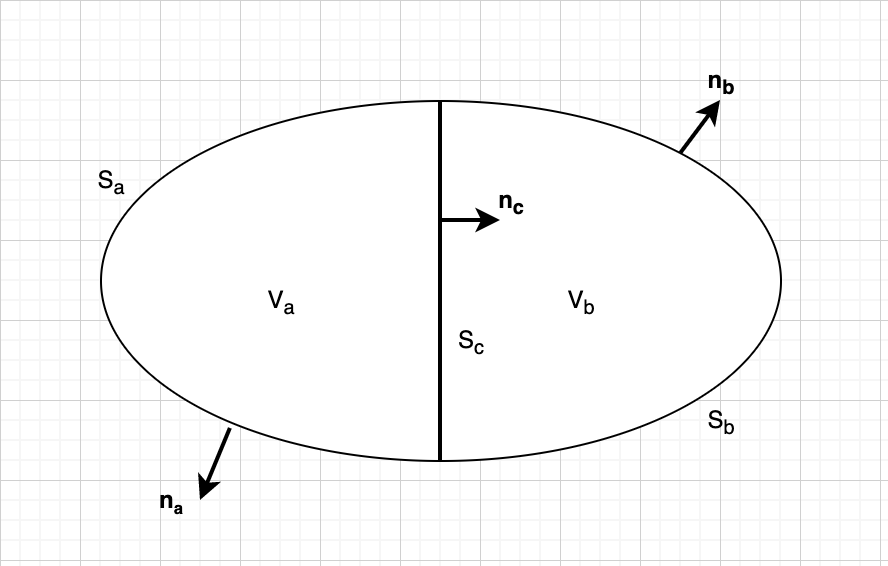
\includegraphics[width=0.7\linewidth]{Materials/Conservation}
	\caption{Illustration of a global volume getting split introducing a new common surface.}
	\label{conservation}
\end{figure}

\subsection{Control volumes}
An integral part of FVM is the control volumes. Control volumes are introduced as part of our discretization to simplify our problem such that we look at a local subproblem which is easier to solve. Control volumes can be of any shape as long as we have the geometric information of them, e.g. cell centers, surface centers, neighbouring cells, surface connectivity etc. For this week's assignment we will construct a regular triangle mesh. In this mesh we will define the control volumes 'around' vertices of the mesh. That is, in the interior of the mesh we will construct octagons and squares going between the centers of our triangle mesh. At the boundaries of our mesh we will create polygons. This can be seen in \autoref{controlvolume}. Although there are no formal requirements on the shape of the control volumes we need the edges of the control volumes to be perpendicular to the grid lines in our mesh, otherwise the outwards unit normal of the control volume surface will point in a different direction than the line segments connecting our vertices and we will introduce errors in our later approximations. Because of this we need to tailor the shape of our control volumes such that they match with our choice of mesh.

\subsection{FVM applied to Magnetostatic problem}
We can now apply FVM to our problem in this week's notebook, namely the Magnetostatic problem which has the PDE $\nabla \cdot \nabla \phi(\mathbf{x}) = \nabla \cdot \mathbf{M}(\mathbf{x})$. The first step of FVM is to decide on a mesh and control volume layout. As we are dealing with a 2D problem in the notebook we will use a regular triangle mesh. For control volumes we will use the centers in the triangles to draw octagons and squares between interior nodes, and simple lines to the boundary. This is illustrated in \autoref{controlvolume} where black lines is our mesh and red lines constitute our control volumes. The next step is to convert our PDE to a volume integral and then to a surface integral using the \textit{Gauss-Divergence theorem}.
\begin{align*}
	\nabla \cdot \nabla \phi(\mathbf{x}) &= \nabla \cdot \mathbf{M}(\mathbf{x})\\
	\int_V\nabla \cdot \nabla \phi(\mathbf{x})dV &= \int_V \nabla \cdot \mathbf{M}(\mathbf{x})dV\\
	\int_S\nabla \phi(\mathbf{x})\cdot \mathbf{n}dS &= \int_S \mathbf{M}(\mathbf{x})\cdot \mathbf{n}dS
\end{align*}
Where $\mathbf{n}$ is the outward unit normal. These surface integrals means we need to integrate over the edges of our control volumes. We can now exploit that the edges are piecewise continuous, making our integrals \textit{piecewise continuous integrals}. 
\begin{equation*}
	\sum_e\int_{S_e}\nabla \phi(\mathbf{x})\cdot \mathbf{n_e}dS = \sum_e\int_{S_e} \mathbf{M}(\mathbf{x})\cdot \mathbf{n_e}dS
\end{equation*}
Where $\mathbf{n_e}$ denotes the outward unit normal for the edges in the control volume. We can now use the midpoint approximation rule to remove the integral. This can be done because the outward unit normal is constant along each $S_e$ part. 
\begin{equation*}
		\sum_e[\nabla \phi(\mathbf{x})\cdot \mathbf{n_e}]_cl_e = \sum_e [\mathbf{M}(\mathbf{x})\cdot \mathbf{n_e}]_cl_e
\end{equation*}
Here $l_e$ denote the length of the control volume edge we are looking at. To approximate $[\nabla \phi(\mathbf{x})\cdot \mathbf{n_e}]_c$ we realise we can rewrite it as a directional derivative. We note because of the way we have defined our control volumes we have $n_e$ points in the same direction as the line segment between two vertices and we can thus make the approximation:
\begin{equation*}
	\nabla\phi(\mathbf{x})\cdot \mathbf{n_e} = \frac{\partial\phi(\mathbf{x})}{\partial \mathbf{n_e}} \approx \frac{\phi(\mathbf{x})_j - \phi(\mathbf{x})_i}{l_{ij}}
\end{equation*}
Where $\phi(\mathbf{x})_i$ is the $\phi$ value at a vertex \textit{i} in our mesh, $\phi(\mathbf{x})_j$ is the $\phi$ value at a vertex \textit{j} in our mesh and $l_{ij}$ is the length of the line segment connecting the two vertices. Substituting this in and cleaning up we end with the discretization:
\begin{align*}
	\sum_e\frac{(\phi(\mathbf{x})_j - \phi(\mathbf{x})_i)}{l_{ij}}l_e &= \sum_e [\mathbf{M}(\mathbf{x})\cdot \mathbf{n_e}]_cl_e\\
	\sum_e\frac{l_e}{l_{ij}}(\phi(\mathbf{x})_j - \phi(\mathbf{x})_i) &= \sum_e [\mathbf{M}(\mathbf{x})\cdot \mathbf{n_e}]_cl_e
\end{align*}
This approximation does however introduce small error along the boundary. This is illustrated in \autoref{boundary} where we end up estimating the $\phi$ value only halfway to the boundary (red dot) instead of at the boundary (green dot) because the control volume edge only goes to the boundary. We could instead use a more complicated approximation where we use shape functions like in FEM to interpolate the value to the boundary. This would mean we would have $\nabla \phi(\mathbf{x}) = \sum_\alpha \nabla N_{\alpha}\hat{\phi}_{\alpha} = \mathbf{N}\hat{\phi}$ where $N_{\alpha}$ is a shape function and $\hat{\phi}$ is a set of discrete $\phi$ values we would then solve for. 

\begin{figure}
	\centering
	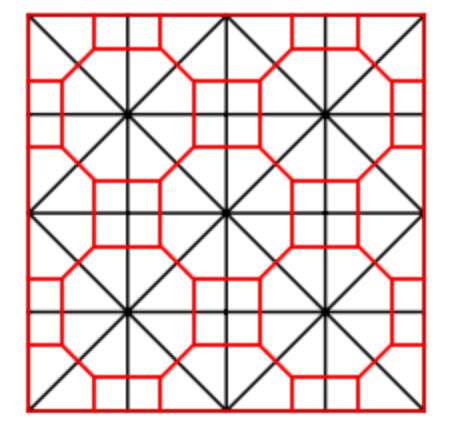
\includegraphics[width=0.5\linewidth]{Materials/ControlVolume}
	\caption{Our mesh drawn in black and our control volumes drawn in red.}
	\label{controlvolume}
\end{figure}

\begin{figure}
	\centering
	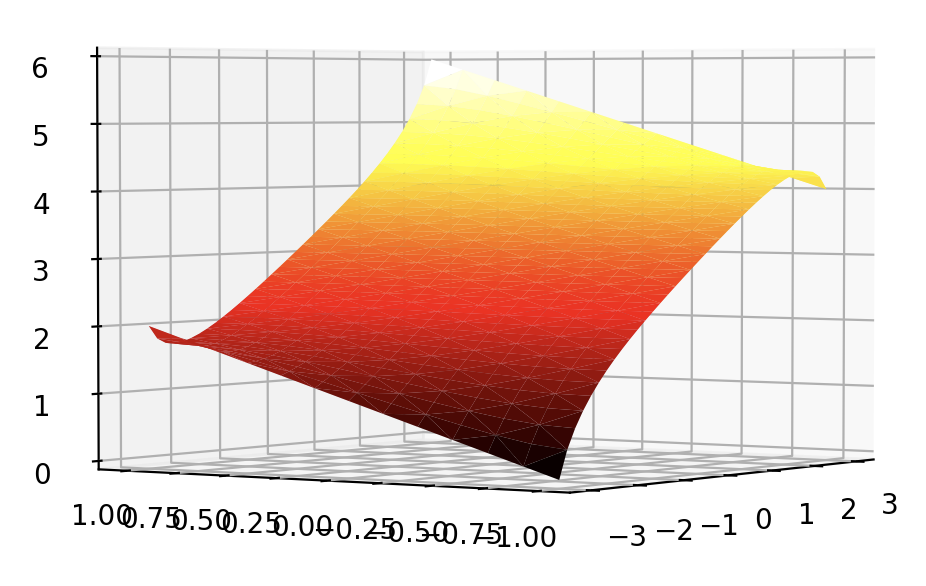
\includegraphics[width=0.5\linewidth]{Materials/boundary}
	\caption{Small error introduced by not using shape functions for interpolation. Blue lines illustrate edges in control volumes and the black lines illustrate a single boundary triangle in our mesh.}
	\label{boundary}
\end{figure}

\subsection{Handling of unit circle}
In this week's assignment when we look at the right hand side integral, $\int_V \nabla \cdot \mathbf{M}(\mathbf{x})dV$, we require the integrand, $\nabla \cdot \mathbf{M}(\mathbf{x})$, to be a continuous real valued function. When we consider a control volume completely outside the unit circle $\mathbf{M}(\mathbf{x})$ is per definition $[0,0]^T$ and thus continuous. When we consider a control volume completely inside the unit circle $\mathbf{M}(\mathbf{x})$ is per definition $[0,-1]^T$ and thus also continuous. However, when we have a control volume which is partially inside and partially outside then $\mathbf{M}(\mathbf{x})$ suddenly jumps from one value to another and is thus discontinuous. We can handle this by splitting the integral into two parts, one over the part of the control volume which is outside the unit circle, and one which is inside and then sum the two parts. That is we would have:
\begin{equation*}
	\int_V \nabla \cdot \mathbf{M}(\mathbf{x})dV = \int_{V_{inside}} \nabla \cdot \mathbf{M}(\mathbf{x})dV + \int_{V_{outside}} \nabla \cdot \mathbf{M}(\mathbf{x})dV
\end{equation*}
This split can either be done on the fly when we realise our control volume is getting split by the unit circle, or we could preemptively design our control volumes such that their boundaries conforms with the unit circle.
\subsection{Difference between Finite Methods}
FVM resembles some of the same concepts as FEM as in both methods we start with a big system which we then divide into smaller subsystems which we then can solve more easily. However, where FEM uses trial functions and integration by parts to convert from strong form to weak form, FVM takes a more direct approach and uses Gauss-Divergence theorem to get surface integrals. FEM also relies on the approximation from using shape functions to interpolate positions inside the domain, where FVM can make use of shape functions, but can also as seen earlier, make use of the outward unit normal from the control volumes. Comparing to FDM, FVM and FEM are much more easily applied to unstructured meshes as it is not always obvious which nodes to use for FDM in an unstructured mesh. However, FDM can quite easily be formally verified though analysis of the Taylor remainder terms, which is not as obviously done for FVM and FEM.
	\section{Experiments}
	In the following experiments we will look at a 2D problem. We will solve the partial differential equation $\frac{\partial^2 u(p))}{\partial x^2} + \frac{\partial^2 u(p)}{\partial y^2} = c(p)$ where \textit{p} is a point in our domain and $c(p)$ is a known function. From this definition we can see $c(p)$ expresses the curvature of the \textit{u} function which we want to approximate. This means when if we define $c(p) = 0$ we will get a linear plane as a solution, and otherwise our solution will have a curve to it. 
	\section{Experiment 1 - How boundaries affect advection with semi Lagrangian time integration}
In this experiment we would like to examine how the boundaries affect our advection. In this week's notebook we have worked with the peaks functions, and used advection with semi Lagrangian time integration to turn the scalar field 360 degrees around. This can be seen in \autoref{original} and we will use this as a baseline comparison for our experiment.
\begin{figure}[H]
	\centering
	\begin{subfigure}[b]{0.40\linewidth}
		\centering
		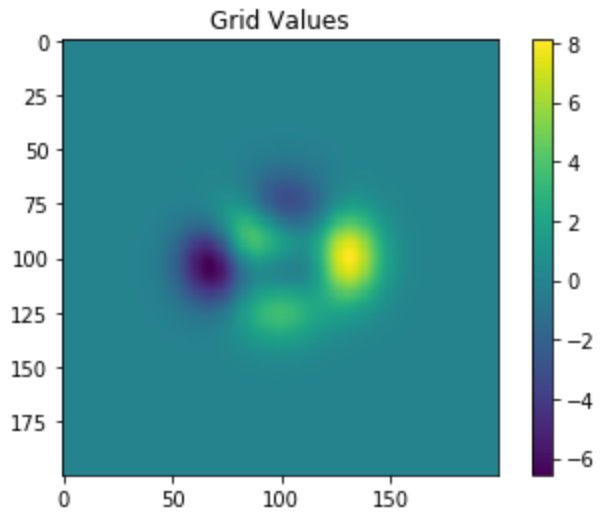
\includegraphics[width=\linewidth]{Materials/Lagrangian/ot0}
		\caption{Image of peaks function before advection.}
		\label{ot0}
	\end{subfigure}
	\hfill
	\begin{subfigure}[b]{0.40\linewidth}
		\centering
		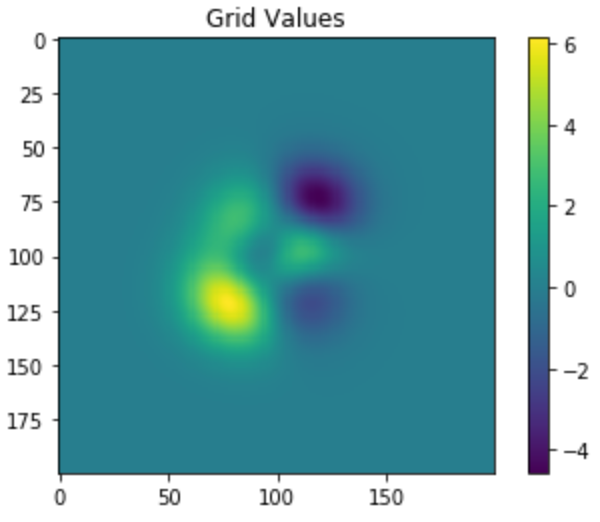
\includegraphics[width=\linewidth]{Materials/Lagrangian/ot1}
		\caption{Image of peaks function after $\frac{1}{2}\pi$ rotation.}
		\label{ot1}
	\end{subfigure}
	\\
	\begin{subfigure}[b]{0.40\linewidth}
		\centering
		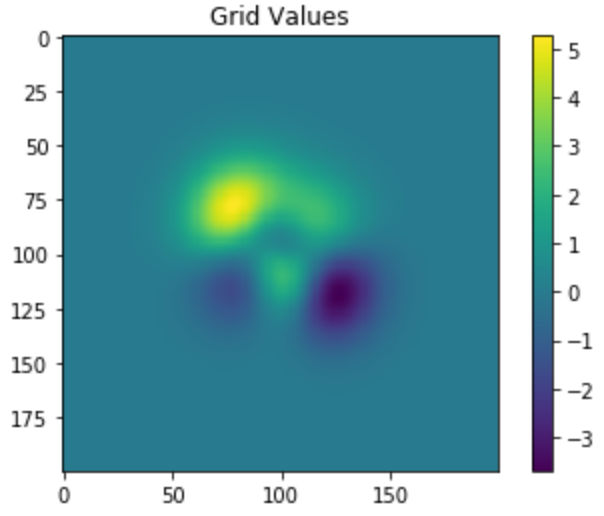
\includegraphics[width=\linewidth]{Materials/Lagrangian/ot2}
		\caption{Image of peaks function after $1\frac{1}{1}\pi$ rotation.}
		\label{ot2}
	\end{subfigure}
	\hfill
	\begin{subfigure}[b]{0.40\linewidth}
		\centering
		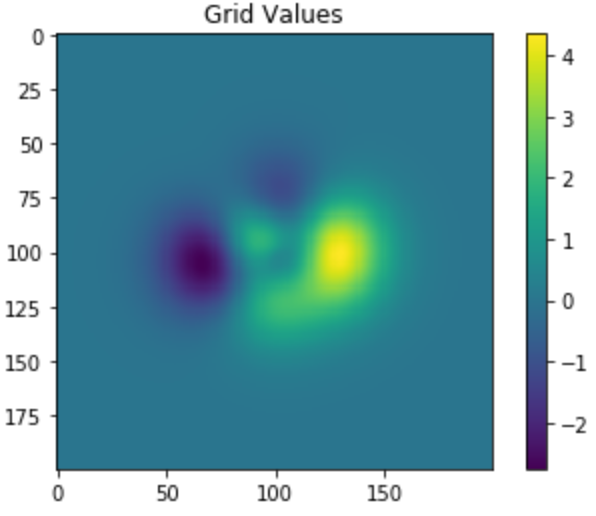
\includegraphics[width=\linewidth]{Materials/Lagrangian/ot3}
		\caption{Image of peaks function after $2\pi$ rotation.}
		\label{ot3}
	\end{subfigure}
	\caption{Advection without any boundary issues. The grid is defined over the domain $-5$ to $5$ with 200 grid nodes along each axis, and with $\Delta t = 0.0005$.}
	\label{original}
\end{figure}
As we see this is no perfection advection, and we have an error of $0.21$, meaning we loose about $21\%$ mass. We also note we are not having any issues with boundaries, as the peaks rotate in the middle of the grid without hitting the boundaries. We can now shrink the grid such that when rotating the peaks we will move outside the grid. The previous grid was defined over the domain $-5$ to $5$, we now shrink this to $-1.5$ to $1.5$.
\begin{figure}
	\centering
	\begin{subfigure}[b]{0.40\linewidth}
		\centering
		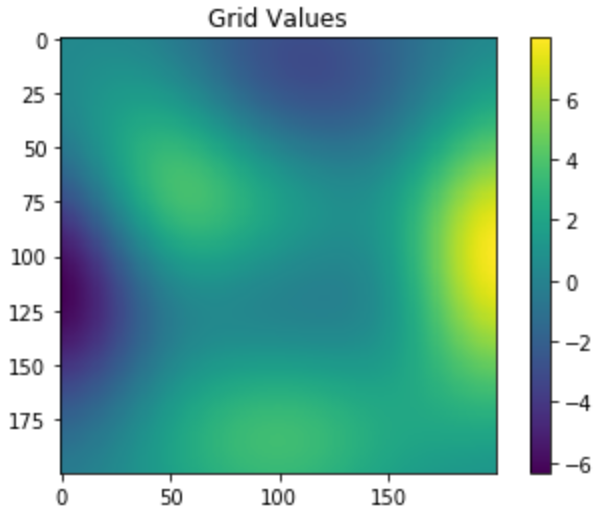
\includegraphics[width=\linewidth]{Materials/Lagrangian/et0}
		\caption{Image of peaks function before advection.}
		\label{et0}
	\end{subfigure}
	\hfill
	\begin{subfigure}[b]{0.40\linewidth}
		\centering
		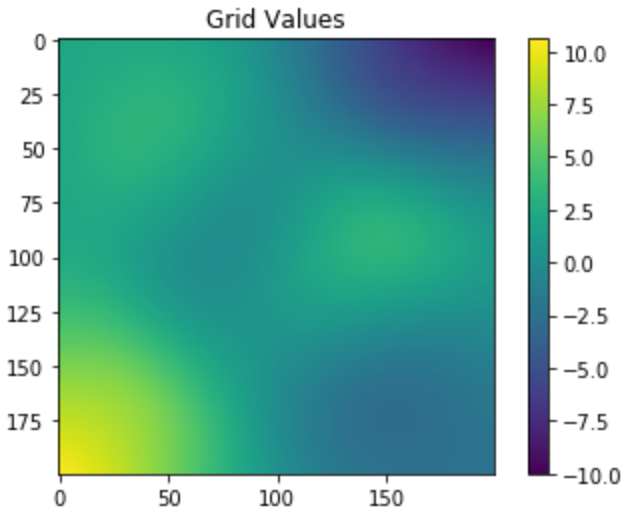
\includegraphics[width=\linewidth]{Materials/Lagrangian/et1}
		\caption{Image of peaks function after $\frac{1}{2}\pi$ rotation.}
		\label{et1}
	\end{subfigure}
	\\
	\begin{subfigure}[b]{0.40\linewidth}
		\centering
		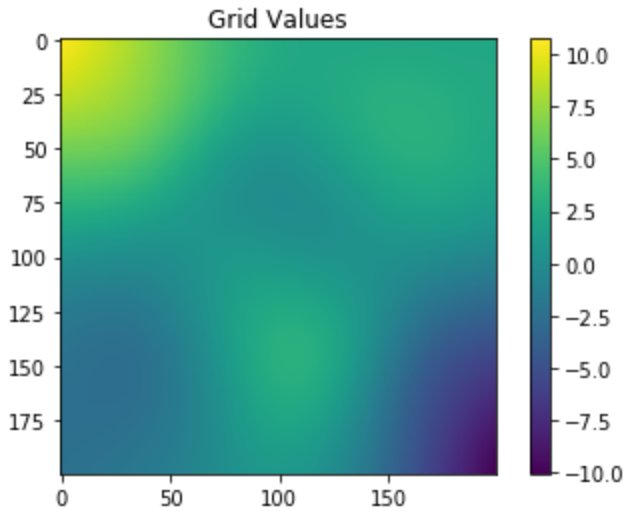
\includegraphics[width=\linewidth]{Materials/Lagrangian/et2}
		\caption{Image of peaks function after $1\frac{1}{1}\pi$ rotation.}
		\label{et2}
	\end{subfigure}
	\hfill
	\begin{subfigure}[b]{0.40\linewidth}
		\centering
		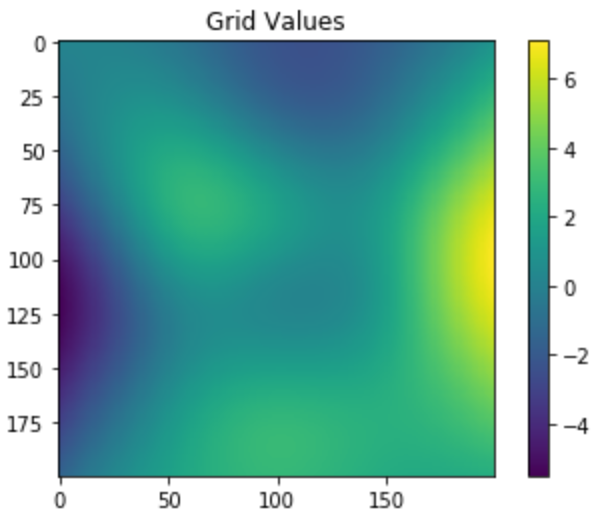
\includegraphics[width=\linewidth]{Materials/Lagrangian/et3}
		\caption{Image of peaks function after $2\pi$ rotation.}
		\label{et3}
	\end{subfigure}
	\caption{Advection with boundary issues. The grid is defined over the domain $-1.5$ to $1.5$ with 200 grid nodes along each axis, and with $\Delta t = 0.0005$.}
	\label{experiment1}
\end{figure}
In \autoref{experiment1} we see the results of shrinking the grid. When comparing \autoref{ot0} and \autoref{et0} we do not see too much of a difference except we have 'zoomed in'. However, comparing \autoref{ot1} with \autoref{et1} and \autoref{ot2} with \autoref{et2} we see that the 'shapes' are similar, but that the peaks have become a lot larger in the corners of \autoref{et1} and \autoref{et2} and similarly the big canyon have becomes much deeper. This is to the extend that the smaller peaks in the experiment images have grown almost as large as the original large peak. We also see that the small canyon in the lower right corner of \autoref{et1} and lower left corner of \autoref{et2} have been somewhat leveled out. When comparing \autoref{ot3} and \autoref{et3} we see pretty much the same shapes but we again see the scaling of the peaks have changed, although not as drastically as for the intermediate rotations.

\subsection{Discussion of results}
We see when we shrink the domain that instead of the peaks and canyons going towards 0 they actually become bigger. As they rotate, they move outside our grid, and thus we need to interpolate them back in. In this process we compute the new grid value based on an interpolation to the nearest grid cell. The fact we move outside the grid causes us to lose information about the peaks and canyons and because we use the neighbourhood around the nearest grid cell we also a slight error in the computed value as it actually should have been computed at a slightly different location. These are probably the causes we see a different behaviour of the peaks and canyons compared to when we do not have any boundary issues. The interpolation used to get the results for this experiment is the interpolation function in this week's notebook.

	\section{Experiment 2}
In this experiment we would like to experimentally verify that our simulation gets more accurate as we increase the mesh resolution. We will do this by applying light gravitational force to a cantilever beam fixed to a wall. We then measure the position of a lowest hanging vertex as we increase the mesh resolution. In the real world gravity would be applied to all molecules, and so our expectation is the measured position converge towards some fixed value as the simulation gets more realistic with more nodes. Our initial grid resolution will be 12x4, and we will then increase the mesh resolutions in multiples of this initial resolution. The results can be seen in \autoref{positions}.
\begin{figure}
	\centering
	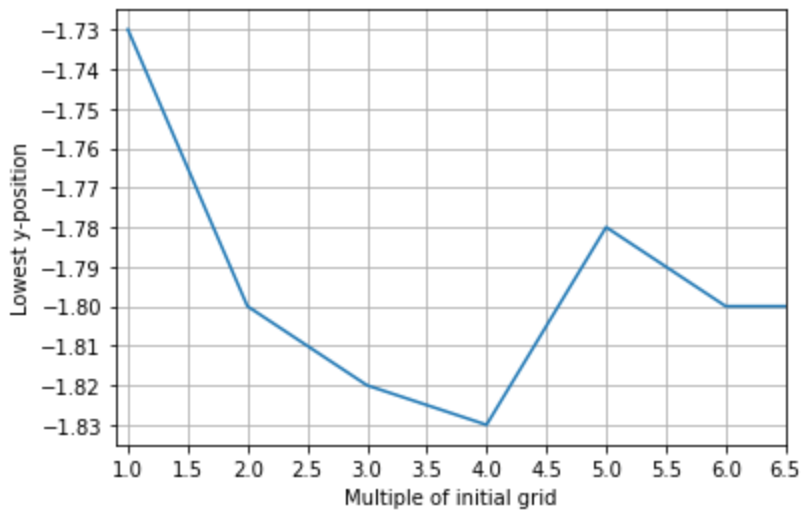
\includegraphics[width=0.9\linewidth]{Materials/positions}
	\caption{Lowest vertex position of the simulation measured for different mesh resolutions.}
	\label{positions}
\end{figure}

\subsection{Discussion of results}
In the beginning we see the lowest positions changes quite a lot as we make the grid finer, but towards the end it seems the lowest position converges towards $-1.8$. This matches our expectation about fine mesh resolutions would converge towards a fixed value. We thus conclude our discretization of how the forces are applied is correct.
	\section{Conclusion}
In conclusion we have seen where segmentation can be used in medical image analysis, we have seen the risks of dilation and erosion and explained the benefits of them, we have concluded Graph cut segmentations are preferred, but also have limited applications and Random walker alleviates these constrains by being non-deterministic, and finally we have looked into how PCA can be used for segmentation.
	\newpage

	%\bibliography{Exercises/mybib}

	
\end{document}
\endinput
